\section{Ausgleichsrechnung / Interpolation}

Zur Auswertung Datenpunkte mit Streuung durch eine Funktion annähern.

\begin{description}
    \item[Interpolation] eine Funktion die exakt durch die Messpunkte geht.
        Geeignet falls:
        \begin{itemize}
            \item wenig Datenpunkte
            \item (fast) keine Messfehler
        \end{itemize}
    \item[Ausgleichsrechnung] eine Funktion die summiert die kleinste Abweichung
        von den Messpunkten hat. Zwischen den Messpunkten oftmals stabiler
        als Interpolation
        \begin{itemize}
            \item typischerweise viele Datenpunkte
            \item fehlerbehaftet
        \end{itemize}
\end{description}

\section{Interpolation}

\begin{itemize}
    \item Gegeben: \textcolor{red}{$n+1$} Wertepaare $(x_i, y_i), \, i = 0,...,n$ 
        mit $x_i \ne x_j \, | \, i \ne j$
    \item Gesucht: stetige Funktion $g(x)$ mit $g(x_i) = y_i \, \forall i = 0,1,...,n$ \\
        (was zwischen diesen Punkten für Resultate herauskommen kann stark variieren)
\end{itemize}


\subsection{Polynominterpolation}

Zu den $n+1$ Stützpunkten ist ein Polynom $P_n(x) 
    = a_0 + a_1 x + a_2 x^2 + ... + a_n x^n$ vom Grad $n$ gesucht.

Weil das Polynom vom Grad $n$ ist lässt sich zusammen mit den Stützpunkten
ein lineares Gleichungsystem dazu aufstellen.

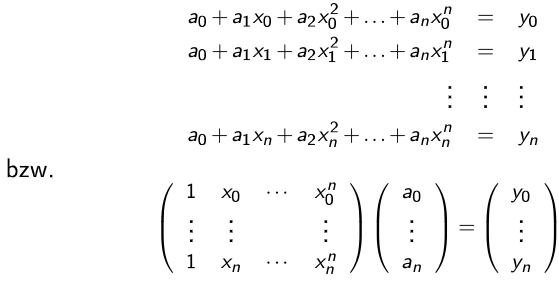
\includegraphics[scale=0.3]{interpol-poly-linearglgs}


\subsubsection{Lagrange Interpolationsformel}

Durch $n+1$ Stützpunkte mit verschiedenen Stützstellen gibt es genau EIN Polynom
$P_n(x)$ vom Grade $\le n$ welches alle Stützpunkte interpoliert.

Lagrangeform für $P_n(x)$:
$$P_n(x) = \sum_{i=0}^n l_i(x) y_i$$

Die Lagrangepolynome vom Grad $n$ ($l_i(x)$) sind definiert durch:
$$l_i(x) = \prod_{j=0, j \ne i}^n \frac{x - x_j}{x_i - x_j} \qquad \qquad i = 0,1,...,n$$

Beispiel:\\
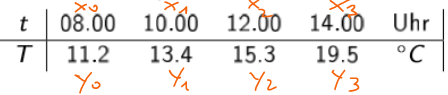
\includegraphics[scale=0.39]{interpol-poly-lagrange-bsp-data} \\
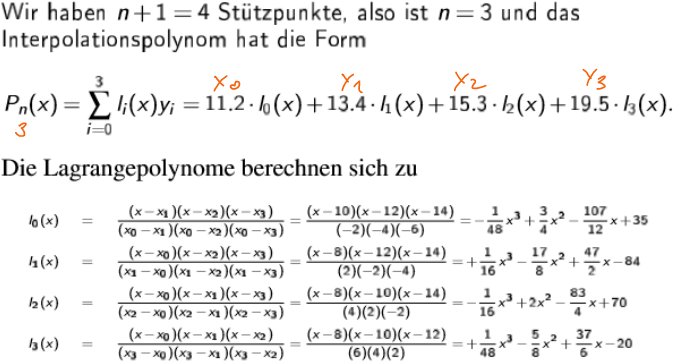
\includegraphics[scale=0.39]{interpol-poly-lagrange-bsp}


\subsubsection{Fehlerabschätzung}

Rein theoretisch weil man die tatsächliche Funktion $f$ kennen müsste.\\
Gegeben $y_i = f(x_i)$ und $f$ genügend oft stetig differenzierbar:

{
\Large
\begin{align*}
 |f(x) - P_n(x)| \quad \le \quad & \frac{|(x-x_0)(x-x_1)...(x-x_n)|}{(n+1)!}\\
                         & * \max_{x_0 \le \xi \le x_n} |f^{(n+1)}(\xi)|
\end{align*}
}



\subsection{Spline-Interpolation}

\subsubsection{Kontext}

Die Annhäherung durch ein einziges Polynom ist zwischen den Messpunkten oft
hoch instabil. Als Alternative kann stattdessen stückweise interpoliert werden.

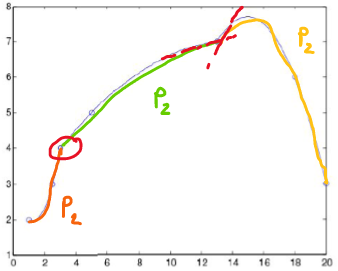
\includegraphics[scale=0.3]{interpol-split-poly-bsp}

\begin{itemize}
    \item hier stören die Knicke(Ableitung verschieden von beiden Seiten) an 
        den Übergängen
    \item die Spline-Interpolation versucht durch Polynome niederen Grades zu 
        interpolieren und damit Schwingungen unterdrücken $\rightarrow$ keine Knicke
    \item Polynome müssen dazu an den Messpunkten nicht nur selben Funktionswert
        sondern auch selbe Ableitung haben (1. und 2. Ableitung).
\end{itemize}

Man kann so für jedes Interval $[x_i, x_{i+1}], \quad i = 0,1,2,...,n-1$ genau 
ein Polynom $s_i$ ansetzen ($i$ Bezeichnet die Nummer des Intervalls).

Dieses Polynom muss folgende Bedingungen erfüllen:
{\large
\begin{description}[itemsep=1mm]
    \item[Interpolation] $s_i(x_i) \, = \, y_i \quad,
        \quad s_{i+1}(x_{i+1}) \, = \, y_{i+1}$
    \item[stetiger Übergang] $s_i(x_{i+1}) \, = \, s_{i+1}(x_{i+1}) \quad,
        \quad s_{i+1}(x_{i+2}) \, = \, s_{i+2}(x_{i+2})$
    \item[keine Knicke] $s'_i(x_{i+1}) = s'_{i+1}(x_{i+1}) \quad,
        \quad s'_{i+1}(x_{i+2}) = s'_{i+2}(x_{i+2})$
    \item[gleiche Krümmung] $s''_i(x_{i+1}) \, = \, s''_{i+1}(x_{i+1}) \quad,
        \quad s''_{i+1}(x_{i+2}) \, = \, s''_{i+2}(x_{i+2})$
    \item[Zusatzbedingungen] Damit es genug Gleichungen für ein reguläres System
        sind müssen noch Zusatzbediungen gesetzt werden, diese unterscheiden sich
        je nach Art des gewählten Splines
\end{description}
}

\subsubsection{natürliche kubische Splinefunktion}
Gegeben $n+1$ Stützpunkte $(x_i, y_i)$ mit monoton aufsteigenden
Stützstellen $x_0 < x_1 < ... < x_n \quad | \quad \mathrm{und}\; n \ge 2$
Gesucht natürliche kubische Splinefunktion $S(x)$, in jedem Intervall $[x_i, x_{i+1}]\, ,\,i=0,1,...,n-1$



Beispiel (6.5 in Folien):\\
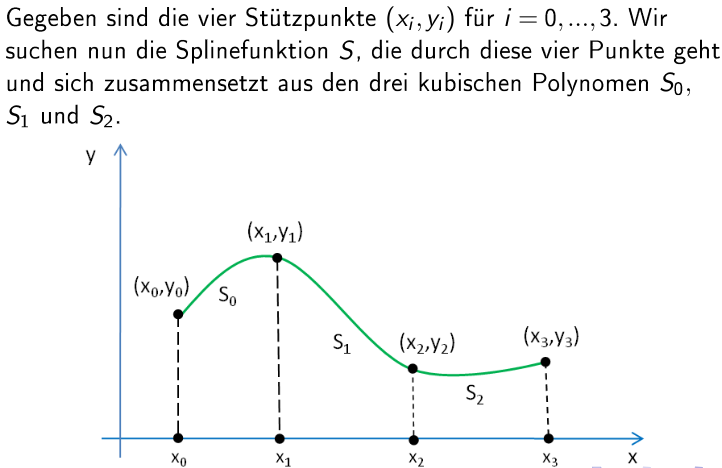
\includegraphics[scale=0.3]{interpol-spline-bsp-ausgang}\\
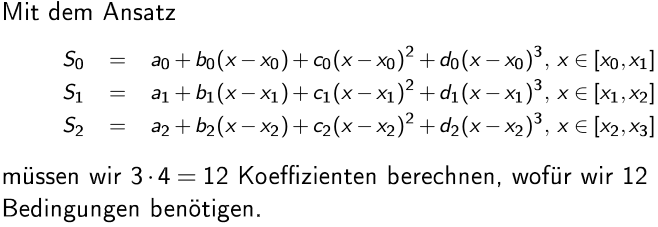
\includegraphics[scale=0.3]{interpol-spline-bsp-ansatz}\\
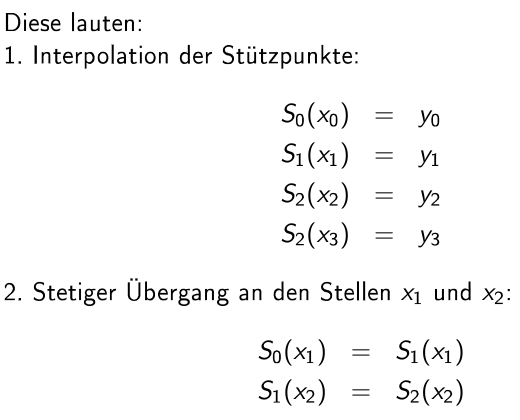
\includegraphics[scale=0.3]{interpol-spline-bsp-bedingungen1}\\
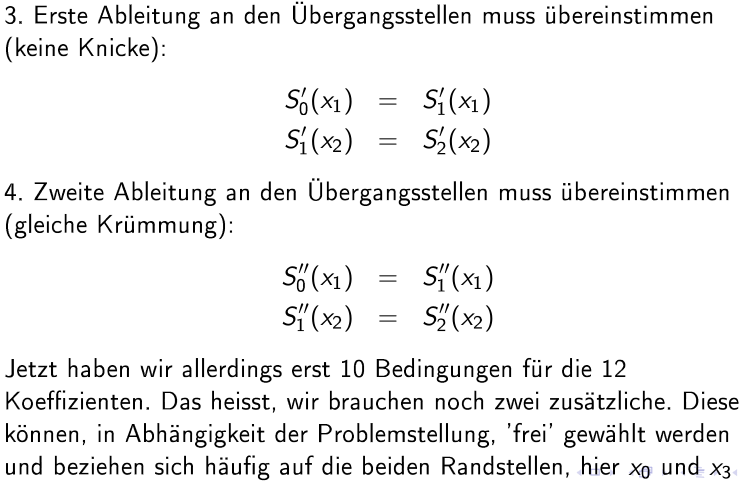
\includegraphics[scale=0.3]{interpol-spline-bsp-bedingungen2}\\
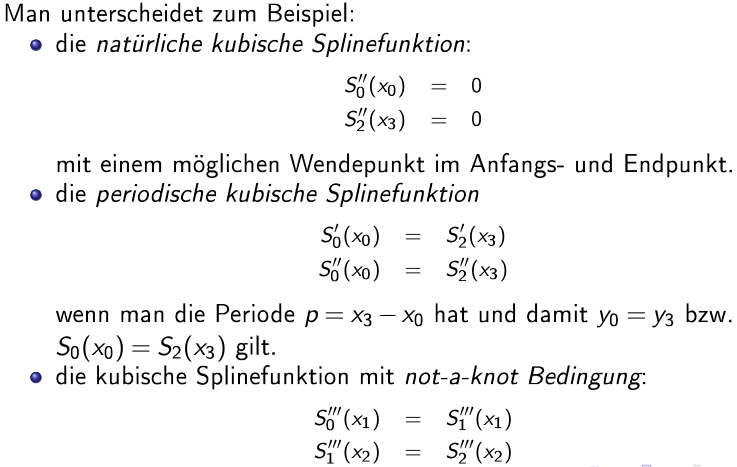
\includegraphics[scale=0.3]{interpol-spline-bsp-zusatzbedingungen}\\









